% This is samplepaper.tex, a sample chapter demonstrating the
% LLNCS macro package for Springer Computer Science proceedings;
% Version 2.20 of 2017/10/04
%
\documentclass[runningheads]{llncs}
%
\usepackage{graphicx}
\usepackage{amstext,amsmath,amssymb,bm,mathtools}

\newtheorem{ddef}{Definition}
\DeclareMathOperator*{\argmin}{arg\,min}
\DeclarePairedDelimiter\norm{\lVert}{\rVert}%
\DeclarePairedDelimiter\abs{\lvert}{\rvert}%

% Used for displaying a sample figure. If possible, figure files should
% be included in EPS format.
%
% If you use the hyperref package, please uncomment the following line
% to display URLs in blue roman font according to Springer's eBook style:
% \renewcommand\UrlFont{\color{blue}\rmfamily}

\begin{document}
%
\title{Digital Curvature Boundary Correction\thanks{This  work has  been  partly  funded by CoMeDiC ANR-15-CE40-0006 research grant.}}

\author{Daniel Antunes\inst{1}
Jacques-Olivier Lachaud\inst{1}
Hugues Talbot\inst{2}}
%
\authorrunning{D. Antunes et al.}
% First names are abbreviated in the running head.
% If there are more than two authors, 'et al.' is used.
%
\institute{Laboratoire de Mathematiques (LAMA), Universite Savoie Mont Blanc, Chambéry, France
\email{daniel.martins-antunes, jacques-olivier.lachaud@univ-savoie.fr} \and
CentraleSupelec Université Paris-Saclay\\
\email{hugues.talbot@centralesupelec.fr}}
%
\maketitle              % typeset the header of the contribution
%
\begin{abstract}
Recent works indicates the potential of curvature as a regularizer in image segmentation, in particular for the class of thin and elongated objects, ubiquitous in medical imagery, in which length regularization performs badly. Howerver, state-of-art techniques make use of a coarse approximation of curvature  limiting its practical applications. We argue that curvature must be computed using a multigrid convergent estimator, instead. As an illustration, we propose a two-stage method based on the minimization of a squared curvature energy that enhances the output quality of grab-cut image segmentation.
 
\keywords{Multigrid convergence  \and Digital estimator \and Curvature \and Optimization.}
\end{abstract}
%
%
%

\section{Introduction}
Geometric quantities are particularly useful as regularizers, specially when object geometry is known a priori. Length is a general purpose regularizer and the literature is vast on models that make use of it \cite{casseles97},\cite{appleton05}. However, length is not suitable to segmentation of thin and elongated objects, as it is propense to oversegmentation. Such drawback can be overcomed by injecting curvature regularization \cite{zehiry10}.
				
One of the first successful uses of curvature in image processing is the inpainting algorithm described in \cite{masnou98}. The author evaluates the elastica energy along the level lines of a simply-connected image to reconstruct its occluded parts. The level lines property of non-intersection allows the construction of an efficient dynamic programming algorithm. Nonetheless, it is still a challenging task to inject curvature in a image segmentation model. 

The state-of-art methods are difficult to optimize and algorithms  not practical for large images \cite{schoenemann09},\cite{nieuwenhuis14}. Such approaches make use of a coarse and not multigrid convergent approximation of curvature, which is an important drawback.


\section{Multigrid Convergent Estimators}
To be written...\\
Why MGC estimators should be preferred?

\subsection{Integral Invariant Estimator}
Generally, an invariant $\mu$ is a real-valued function from some space $\mathcal{S}$ which value is unnafected by action of some group $\mathfrak{G}$ on the elements of the domain
		
		\begin{align*}
			x \in \mathcal{S}, g \in \mathfrak{G}, \mu(x) = v \longleftrightarrow \mu(g \cdot x ) = v
		\end{align*}
		
		Perimeter and curvature are examples of invariants for shapes on $\mathbb{R}^2$ with respect to the euclidean group (rigid transformations). Definition of integral area invariant and its one-to-one correspondence with curvature is proven in \cite{manay04}.


\begin{ddef}[Integral area invariant]
	Let $X \in \mathbb{R}^2$ and $B_r(p)$ the ball of radius $r$ centered at point $p$. Further, let $\lambda(\cdot)$ be the characteristic function of $X$. The integral area invariant $\alpha_{X,r}(\cdot)$ is defined as
	
	\begin{align*}
		\forall p \in \partial X, \quad \alpha_{X,r}(p) = \int_{B_r(p)}{ \lambda(x) dx}.
	\end{align*}
\end{ddef}


	The value $\alpha_{X,r}(p)$ is the intersection area of ball $B_r(p)$ with shape $X$. By locally approximating the shape at point $p \in X$, one can rewrite the intersection area $\alpha_{X,r}(p)$ in the form of the Taylor expansion \cite{pottman09}
	
		\begin{align*}
			\alpha_{X,r}(p) = \frac{\pi}{2}r^2 - \frac{\kappa(X,x)}{3}r^3 + O(r^4).
		\end{align*}
		
	The curvature of $X$ at point $p$ can be approximated at arbitrarly precision as the radius $r$ approaches to zero by
	
	\begin{align}
		\tilde{\kappa}(p) \coloneqq \frac{3}{r^3}\left( \frac{\pi r^2}{2} - \alpha_{X,r}(p) \right),
		\label{eq:curvature_approximation}
	\end{align}
	
	Such approximation is convenient as one can simply devise a multigrid convergent estimator for area.

	\begin{ddef}	
		Given a digital shape $D \subset \frac{1}{h} \cdot \mathbb{Z}^2$, a multigrid convergent estimator for area $\widehat{Area}(D,h)$ is defined as	
		
		\begin{align}
			\widehat{Area}(D,h) \coloneqq h^2\text{Card}\left( D \right).			
			\label{eq:digital_estimator_area}
		\end{align}

	\end{ddef}
	
	In \cite{coeurjolly13}, the authors use the approximation\eqref{eq:curvature_approximation} and digital estimator \eqref{eq:digital_estimator_area} to define a multigrid convergent estimator for curvature.

	\begin{ddef}[Integral Invariant Curvature Estimator]
		Let $D \in \frac{1}{h} \cdot \mathbb{Z}^2$ a digital shape and $B_r(p)$ a disk of radius $r$ centered at $p$. The integral invariant curvature estimator is defined as
		
		\begin{align*}
			\hat{\kappa}_{II} \coloneqq \frac{3}{r^3} \left( \frac{\pi r^2}{2} - \widehat{Area} \left( B_{r/h} ( \frac{1}{h} \cdot x ) \cap D, h \right) \right).
		\end{align*}
	\end{ddef}
	

	The estimator is robust to noise and can be extended to estimate the mean curvature of three dimensional shapes.

\section{Digital Boundary Correction}

In the previous section I also need to say a word on Maximal Digital Straight Segments for the estimation of tangent, and in the follow say a word about an estimator for length. Finally, I should argue that the multiplication of two multigrid convergent estimators is multigrid convergent.

Write in terms of cellular complex. Then, define integrated squared curvature using a MGC estimator for length and curvature. We are going to use such definition to evaluate the quality of our method. At each iteration, the energy value should be reduced.

Let $D$ be the digital set representation of a binary image on a cellular grid of size $h$ and $\partial D$ to be its $4$-connected digital set boundary. Further, let $\hat{\kappa}$ to be some digital estimator for curvature. The digital integral squared curvature of $\partial D$ is defined as
		
		\begin{equation}
			E_{k2}(D) \coloneqq  h \cdot \sum_{p \in \partial D}{ \hat{\kappa}^2(p) }.
		\end{equation}
		
		
		Ideally, let $\mathcal{S}(D)$ be the set of digital images similar to $D$ according to some criteria. We wish to find $D^\prime$ such that 

\begin{align}
	D^\prime = \argmin_{x \in \mathcal{S}(D)} E_{k2}(x)\label{eqn:minimum_boundary}
\end{align}
	
	The proposed model uses the integral-based curvature estimator of \cite{coeurjolly13} and the following definition of $\mathcal{S}(D)$.
	
	\begin{align*}
		\mathcal{S}(D) = D \bigtriangleup \partial D.
	\end{align*}
	
	In other words, only boundary points are optimization variables.
	
	\subsubsection{Working example}

	Let $O=\partial D$ be the optimization set and define its complement with respect to $D$ as the fidelity set $F$
	
	\begin{align*}
		F = \left\lbrace x \mid x \in D - O \right\rbrace
	\end{align*}
	
	\begin{figure}[!ht]
		\center
		\includegraphics[scale=0.25]{images/qbo_regions.eps}
		\caption{Optimization set is colored in gray; fidelity set in green.}
	\end{figure}
	
	We use the integral invariant estimator $\hat{\kappa}_{II}$ to estimater the squared curvature value at point $p$.
	
	\begin{align}
		\hat{\kappa}^2(p) = \left( \; \frac{3}{r^3}\left( \frac{\pi r^2}{2} - \alpha_{D,r}(p) \right) \; \right)^2.
		\label{eq:squared_curvature_estimator}
	\end{align}
	
	Further, let $O_{p} \subset O$ to be the subset of optimization variables intersecting with $B_r(p)$. The subset $F_p$ is defined analogously. The factor $A_{r,h}$ can be decomposed in two other terms representing the contribution of points in the fidelity and optimization set.
	
	\begin{align*}
		\alpha_{D,r}(p) = |F_{p}| + \sum_{x \in O_p}{x},
	\end{align*}
	
	Let $Q \coloneqq \frac{\pi r^2}{2}$. Reorganizing terms in \eqref{eq:squared_curvature_estimator} and ignoring the constants 
	
	\begin{align*}
		E_{k2}(p) &= \left( \; \sum_{x_i \in O_{p}}{x_i} \; \right) ^2 -2 \cdot Q\cdot \sum_{x_i \in O_{p}}{x_i} + 2 |F_p| \cdot \sum_{ x_i \in O_{p} }{x_i} \\[1em]
		&= \sum_{x_i \in O_{p}}{x_i^2} + 2 \cdot \sum_{ \substack{ i<j \\ x_i,x_j \in O_{p}  } }{x_ix_j} \quad - 2 (Q-|F_p|)\cdot \sum_{x_i \in O_{p}}{x_i}
	\end{align*}
	
	Which can be further simplified by using the binary character of the variables.
	
	\begin{align*}
		E_{k2}(p) =\sum_{ \substack{ i<j \\ x_i,x_j \in O_{p}  } }{x_ix_j} \quad  - \;(Q-|F_p|-1/2)\cdot \sum_{x_i \in O_{p}}{x_i}
	\end{align*}	
	
	The optimization problem is finally stated as
	
	\begin{equation}
		\min_{x \in O} \sum_{p \in \partial D}E_{k2}(p)
		\label{eq:optimization_problem_no_conn}
	\end{equation}
	
	Minimizing a non-submodular energy is a NP-hard problem, which restrict ourselves to heuristics and approximation algorithms. The QPBO method \cite{kolmogorov07} transforms the original problem in a max-flow/min-cut problem and returns a full optimal labeling for submodular energies. For non-submodular energies (our case) the method is guaranteed to return a partial labeling with the property that the set of labeled variables is part of an optimal solution. 
	
	The proposed model aims to decide which pixels should be kept and which ones should be removed from the currrent boundary by solving \eqref{eq:optimization_problem_no_conn}. Labeled one pixels indicate regions of high positive curvature (see figure \ref{fig:naive_solution})	while zero labeled pixels may indicate concavities or regions of low curvature. Accordingly to the II estimator, we should pull the estimating ball towards the boundary in regions of positive curvature and push it away from regions of negative curvature. We implement such behavior by respectively removing and keeping points on the current boundary.
	
	
	\begin{figure}[!ht]
		\center
		
\includegraphics[scale=2.0]{images/qbo_1D_naive_solution_noneigh.png}
		\caption{Labeled one pixels (white) indicate high positive curvature regions.}
		\label{fig:naive_solution}
	\end{figure}	
	
		Regions of high negative curvature are identified by applying the model on the negative of the input image. The algorithm is summarized in []. Notice that the method keep unlabeled pixels in the boundary.
		
		During experiments, the number of unlabeled pixels was decreased by applying the estimating ball over all image points. The optimization energy in \eqref{eq:optimization_problem_no_conn} is rewritten as
		
	\begin{equation}
		\min_{x \in O} \sum_{p \in D}E_{k2}(p)
	\end{equation}			

\section{Results}

\section{Conclusion}


%
% ---- Bibliography ----
%
% BibTeX users should specify bibliography style 'splncs04'.
% References will then be sorted and formatted in the correct style.
%
\bibliographystyle{splncs04}
\bibliography{bibliography}

\end{document}
